


\section{Related Works}
\subsection{Untimed Stochastic Workflow Nets (USWN)}\label{subsec:spn}
We consider a specific case of Untimed Stochastic Petri Nets, such as Workflow Networks over $k$-bounded Place-Transitions Nets \cite{MarsanCB84,Desel1998,RoggeSoltiAW13}. Untimed Stochastic Petri Nets are tuple $USWN=(P,T,F,\omega,W,i,f)$ where:
\begin{itemize}
\item $P$ is a set of \textit{places} to which we can associate a finite number of indistinguishable tokens.
\item $T$ is a set of \textit{transitions} $t\in T$, to which we associate a label $\lambda(t)\in\Sigma$, where $\Sigma$ also includes the empty string\footnote{Given that we are going to denote the traces as $\tau$ and $t$ as the Petri Net Transitions, we choose to denote the empty string as such instead of $\tau$ as in current literature from Petri Nets.} $\varepsilon$.
\item $F\subseteq (P\times T)\cup (T\times P)$ is a set of arcs. %to which we associate a \textit{firing cost} $\omega\colon F\to\mathbb{N}$.
\item $W\colon T\to \mathbb{R}^+_{>0}$ defines a \textit{firing weight} associated to each transition. 
\item The initial place $i\in P$ has no ingoing edges ($\not\exists t\in T. (t,i)\in F$).
\item The final place $f\in P$ has no outgoing edges ($\not\exists t\in T. (f,t)\in F$).
\end{itemize}
A \textit{marking} is an assignment of a given amount of indistinguishable tokens to places described by a vector $M\colon P\to \mathbb{N}$. We say that a given transition $t$ is \textit{enabled} if $M(p)\geq 1$ for each ingoing $p$ to $t$ ($(p,t)\in F$). If such transition is enabled, then it can \textit{fire} a token. The \textit{enabling transitions} $E(M)$ for a given marking $M$ are all the $t$ reachable from $p$ ($(p,t)\in F$) with $M(p)\neq 0$ where $t$ is enabled. When $t$ can fire a token for a marking $M$, we can generate a novel marking $M'$ from $M$ by moving the tokens from the ingoing places towards the outgoing places as follows:
\[\forall p\in P.\; M'(p)=M(p)-\mathbf{1}_{(p,t)\in F}+\mathbf{1}_{(t,p)\in F}\]
We denote the transition from marking $M$ to marking $M'$ via an enabling $t$ as a relation $M\overset{t}{\to}M'$. We say that a USWN with initial marking $M$ is $k$-\textit{bounded} if each of the markings $M'$ reachable from $M$, $M$ included, have $\forall p\in P.\; M(p)\leq k$\\

\begin{figure}[!t]
	\centering
	\subfloat[An Untimed Stochastic Petri Net.]{\label{fig:spn}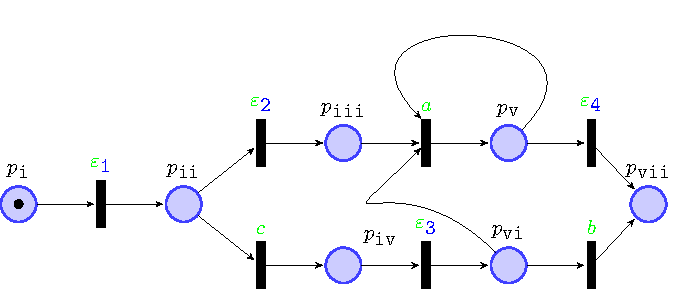
\includegraphics[width=.45\textwidth]{images/petri.pdf}}\quad\subfloat[Reachability Graph associated to the Untimed Stochastic Petri Net.]{\label{fig:rg}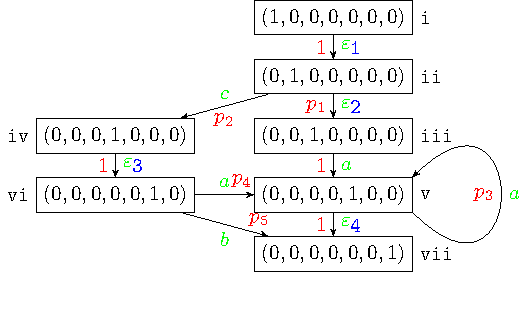
\includegraphics[width=.3\textwidth]{images/rg.pdf}}\\
	\subfloat[Reachability Graph Transformed as a Transition Graph.]{\label{fig:lmc}\label{fig:orig}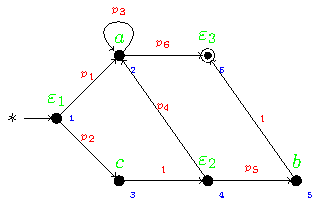
\includegraphics[width=.45\textwidth]{images/running_example.pdf}}\subfloat[Transition Graph after $\varepsilon$-closure.]{\label{fig:closed}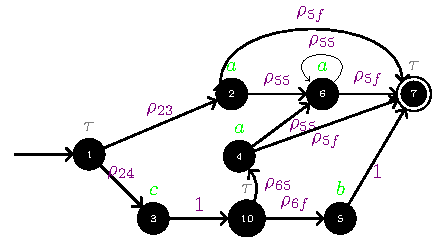
\includegraphics[width=.45\textwidth]{images/closed_example.pdf}}
	\caption{Steps required to transform the set of probabilistic traces associated to a Untimed Stochastic Petri Net into a Transition Graph.}
	\label{transformspn}
\end{figure}
\begin{example}
Figure \ref{fig:spn} provides an example of a Stocastic Petri Net defined as such, and \ref{fig:rg} provides its associated Reachability Graph. This representation can be beneficial when such USWNs are inferred and extracted from log files \cite{PPNFromLog} for extracting the set of the probabilistic traces associated to the USWN.
\end{example}


We use USWNs for modelling business processes: in fact, it can be shown \cite{RaedtsPUWGS07} that it is always possible to convert BPMNs to USWNs. Last, we also assume that a transition is enabled when all of its input places contain at least one token and that, when a transition fires, we remove one token from each of its input places and depose tokens for each of its output places.



\subsection{Transition Graphs (TGs)}\label{subsec:ppn}
Current graph embedding and trace embedding literature uses a different representation of graphs, where nodes (and not edges) are labelled, and where edges are still associated to a transition probability value.

Given a finite set of labels $\Sigma$ and a finite set of nodes $V\subset \mathbb{N}$,  a \textsc{(Probabilistic) Transition Graph} $(s,t,L,R,\omega)$ \cite{GartnerFW03} can be uniquely be described by a initial node $s\in V$, an accepting node $t\in V$, its labels, and a {Markov Chain having} $R$ as a transition matrix. The label matrix is defined by $[L]_{{\color{green}\alpha}\texttt{\color{blue}i}}=1\Leftrightarrow {\color{green}\alpha}=\textit{label}(\texttt{\color{blue}i})$ and $[L]_{{\color{green}\alpha}\texttt{\color{blue}i}}=0$ otherwise, and the transition matrix is defined by the probability $[R]_{\texttt{\color{blue}ij}}$ that the process will, when in node $\texttt{\color{blue}i}$, make a transition into node $\texttt{\color{blue}j}$ \cite{Prob} with $\sum_{\texttt{\color{blue}j}\in V}[R]_{\color{blue}\texttt{ij}}=1$. $[R^n]_{\texttt{\color{blue}ij}}$ denotes the probability of having a path $\texttt{\color{blue}i}\overset{n}{\rightsquigarrow}\texttt{\color{blue}j}$ of length $n$: therefore, $[\Lambda^n]_{\color{green}\alpha\beta}:=[LR^nL^t]_{\color{green}\alpha\beta}/[LL^t]_{\color{green}\alpha\alpha}$ denotes the probability that, having started at any node labelled $\color{green}\alpha$ and taking $n$ steps, we arrive at any node labelled $\color{green}\beta$ (${\color{green}\alpha}\overset{n}{\rightsquigarrow}{\color{green}\beta}$). We denote as ${\color{green}\alpha}{\rightsquigarrow}{\color{green}\beta}$ an aforementioned path of arbitrary length. 
We can also associate a weight $\omega\in[0,1]\subseteq\mathbb{R}$ to a TG, so to express the probability associated with the TG itself as valid. 





\begin{example}
We can graphically represent such TG as in \cite{Myers1989}. 
Figure \ref{fig:orig} is a  TG $P^*=(\mathtt{\color{blue}1},\mathtt{\color{blue}8},L,R,1)$ where $\omega=1$, where the matrices $L$ and $R$ can be both defined as follows:
$$L:=\kbordermatrix{
             & \texttt{\color{blue}1}&\texttt{\color{blue}2}&\texttt{\color{blue}3}&\texttt{\color{blue}4}&\texttt{\color{blue}5}&\texttt{\color{blue}6}&\texttt{\color{blue}7}&\texttt{\color{blue}8}&\texttt{\color{blue}9}&\texttt{\color{blue}10}\\
\color{green}\varepsilon  & \textbf{1}&0&0&0&0&0&\textbf{1}&\textbf{1}&\textbf{1}&\textbf{1}\\
\color{green}a            & 0&\textbf{1}&0&\textbf{1}&0&\textbf{1}&0&0&0&0\\
\color{green}b            & 0&0&0&0&\textbf{1}&0&0&0&0&0\\
\color{green}c            & 0&0&\textbf{1}&0&0&0&0&0&0&0\\
}\qquad R:=\kbordermatrix{
& \texttt{\color{blue}1}&\texttt{\color{blue}2}&\texttt{\color{blue}3}&\texttt{\color{blue}4}&\texttt{\color{blue}5}&\texttt{\color{blue}6}&\texttt{\color{blue}7}&\texttt{\color{blue}8}&\texttt{\color{blue}9}&\texttt{\color{blue}10}\\
\texttt{\color{blue}1}  & 0&0&{\color{red}p_2}&0&0&0&0&0&{\color{red}p_1}&0\\
\texttt{\color{blue}2}  & 0&0&0&0&0&{\color{red}p_3}&{\color{red}p_6}&0&0&0\\
\texttt{\color{blue}3}  & 0&0&0&0&0&0&0&0&0&{\color{red}1}\\
\texttt{\color{blue}4}  & 0&0&0&0&0&{\color{red}p_3}&{\color{red}p_6}&0&0&0\\
\texttt{\color{blue}5}  & 0&0&0&0&0&0&0&{\color{red}1}&0&0\\
\texttt{\color{blue}6}  & 0&0&0&0&0&{\color{red}p_3}&{\color{red}p_6}&0&0&0\\
\texttt{\color{blue}5}  & 0&0&0&0&0&0&0&{\color{red}1}&0&0\\
\texttt{\color{blue}8}  & 0&0&0&0&0&0&0&0&0&0\\
\texttt{\color{blue}9}  & 0&{\color{red}1}&0&0&0&0&0&0&0&0\\
\texttt{\color{blue}10}  & 0&0&0&{\color{red}p_4}&{\color{red}p_5}&0&0&0&0&0\\
}$$
\end{example}

 Given a TG $P=(s,t,L,R,\omega)$, a trace $\tau$ is a tuple in $(\Sigma\backslash\{\varepsilon\})^*$ denoting a path always originating from $s$ and terminating in $t$. 




\subsection{Kernels and Trace Kernels}\label{subsec:katk}
Given a set of data examples $\mathcal{X}$, (e.g., string or traces, TGs) a (positive definite) \textbf{kernel} function $k\colon \mathcal{X}\times \mathcal{X}\to \mathbb{R}$ denotes the similarity of elements in $\mathcal{X}$. If $\mathcal{X}$ is the $d$-dimensional Euclidean Space $\mathbb{R}^d$, the simplest kernel function is the inner product $\Braket{\mathbf{x},\mathbf{x}'}=\sum_{1\leq i\leq d}\mathbf{x}_i\mathbf{x}'_i$. 
A kernel is said to \textbf{perform ideally} \cite{Gartner03} when $k(x,x')=1\Leftrightarrow x=x'$ (\textit{strong equality}) and $k(x,x')=0\Leftrightarrow x\not\simeq x'$ (\textit{strong dissimilarity}). A kernel is also said to be \textbf{appropriate} when similar elements $x,x'\in\mathcal{X}$ are also close in the feature space: appropriateness can be only assessed  empirically \cite{Gartner03}.
Any positive definite kernel induces a distance metric as \cite{Raedt}:
\begin{equation}\label{eq:dofk}
d_k(\mathbf{x},\mathbf{x}'):=\sqrt{k(\mathbf{x},\mathbf{x})-2k(\mathbf{x},\mathbf{x}')+k(\mathbf{x}',\mathbf{x}')}
\end{equation}
When the kernel of choice is the inner product, the resulting distance is the well known Euclidean distance $\norm{\mathbf{x}-\mathbf{x}'}{2}$. A normalized vector (versor) $\hat{\mathbf{x}}$ is defined as $\mathbf{x}/\norm{\mathbf{x}}{2}$: we can easily prove for normalized vectors that $\norm{\hat{\mathbf{x}}-\hat{\mathbf{x}}'}{2}^2=2(1-\Braket{\hat{\mathbf{x}},\hat{\mathbf{x}}'})$.

When $\mathcal{X}$ does not necessarily represent a $d$-dimensional Euclidean space, we can use an \textbf{embedding} $\phi\colon\mathcal{X}\to \mathbb{R}^d$ to define a kernel $k_\phi\colon \mathcal{X}\times \mathcal{X}\to\mathbb{R}$ as $k_\phi(x,x'):=\Braket{\phi(x),\phi(x')}$. As a result, $k_\phi(x,x')=k_\phi(x',x)$ for each $x,x'\in\mathcal{X}$.

Current literature also provides kernel representations for traces (referred as strings in Database literature \cite{LodhiSSCW02,Raedt,GartnerFW03}). We now provide an intuition describing the desired features of such representation \cite{LodhiSSCW02}: if we associate each dimension in $\mathbb{R}^d$ to a different subtrace ${\color{green}\alpha\beta}\in(\Sigma\backslash\{\varepsilon\})^2$ of size $2$ ($2$-grams\footnote{\label{fn:caveat}For our experiments, we choose to consider only $2$-grams, but any $p$-grams of arbitrary length $p\geq 2$ might be considered \cite{Gartner03}. Still, an increased size of $p$ allows to increase precision to the detriment of computational complexity, as all the arbitrary sequences of length $p$ occurring at distance $i<|\tau|$ must be considered.}), the associated coordinate should represent how frequently and ``compatctly'' such subtrace is embedded in the original trace. Therefore, we need to introduce a \textbf{decay factor} $\lambda\in[0,1]\subseteq\mathbb{R}$ weighting the presence of each subtrace ``${\color{green}\alpha\beta}/L$'' as $\lambda^Lm$, where $m$ is the frequency of $\color{green}\alpha\beta$ appearing in the given trace at a distance $L$. Given a trace $\tau\in\Sigma^*$, we can represent it as a TG \cite{Myers1989} $(1,{|\tau|},L_\tau,R_\tau,1)$ having $[L_\tau]_{{\color{green}\alpha}\texttt{\color{blue}i}}=1\Leftrightarrow \tau_{\texttt{\color{blue}i}}={\color{green}\alpha}$ and $[L_\tau]_{{\color{green}\alpha}\texttt{\color{blue}i}}=0$ otherwise, and $\forall i<|\tau|.\; [R_\tau]_{\texttt{\color{blue}i(i+1)}}=1 $ and $[R_\tau]_{\texttt{\color{blue}ij}}=0$ otherwise. Under these assumptions, we can simplify the definition of the embedding from \cite{LodhiSSCW02,Raedt} as $\phi_{\mathcal{T}}(\tau)_{{\color{green}\alpha\beta}}=\sum_{1\leq i\leq |\tau|}\lambda^i[(\Lambda_\tau)^i]_{\color{green}\alpha\beta}$. Please note that this definition is similar to a transition matrix embedding proposed in \cite{GartnerFW03} via geometric series, that is $\sum_i\lambda^i[R^i]_{\color{green}\alpha\beta}$. 

\begin{figure}[!t]
	\centering
	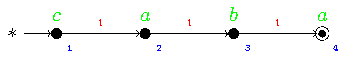
\includegraphics{images/taustar.pdf}
	\caption{Graphical representation of $\tau^*=\textup{caba}$ as a Thompson automaton.}\label{fig:taustar}
\end{figure}
\begin{example}\label{ex:tracembed}
	{Let us suppose that we want to align a trace $\tau^*$ to one of the traces from a transition graph: in order to carry out an approximate alignment, we need to transform it to a transition graph first.} A trace $\tau^*=\textup{caba}$ can be graphically represented in Figure \ref{fig:taustar}. The associated TG $T=(\mathtt{\color{blue}1},\mathtt{\color{blue}4},L,R,1)$ has matrices $L$ and $R$  defined as follows:
	$$L:=\kbordermatrix{
		& \texttt{\color{blue}1}&\texttt{\color{blue}2}&\texttt{\color{blue}3}&\texttt{\color{blue}4}\\
		\color{green}a            & 0&\textbf{1}&0&\textbf{1}\\
		\color{green}b            & 0&0&\textbf{1}&0\\
		\color{green}c            & \textbf{1}&0&0&0\\
	}\qquad R:=\kbordermatrix{
		& \texttt{\color{blue}1}&\texttt{\color{blue}2}&\texttt{\color{blue}3}&\texttt{\color{blue}4}\\
		\texttt{\color{blue}1}  & 0&\color{red}1&0&0\\
		\texttt{\color{blue}2}  & 0&0&\color{red}1&0\\
		\texttt{\color{blue}3}  & 0&0&0&\color{red}1\\
		\texttt{\color{blue}4}  & 0& 0& 0& 0\\
	}$$
We can similarly represent all the traces from the USPN.
\end{example}

%\begin{example}
%The subtrace \textit{\textbf{\uline{hi}}} is represented in \textit{\textbf{\uline{hi}}deous},   \textit{\uline{\textbf{h}}e\uline{{i}}d\textbf{i}}, and \textit{\uline{{\textbf{h}i}}nd\textbf{i}}, but with different frequencies and subtrace distances. We have $\phi_{\mathcal{T}}(\textit{hideous})_{{\color{green}hi}}=\lambda$,  $\phi_{\mathcal{T}}(\textit{heidi})_{{\color{green}hi}}=\lambda^2+\lambda^4$, and $\phi_{\mathcal{T}}(\textit{hindi})_{{\color{green}hi}}=\lambda+\lambda^4$.
%\end{example}



\begin{table}[!t]
\caption{Embedding for both $\tau^*=cacb$ and some traces caaa, caa and cb generated from the USPN $\mathcal{U}$ in Figure \ref{fig:spn}}\label{tb:embedding}
\begin{center}
	\begin{tabular}{l|l|l|l|l|l|l|l|l|l|}
		\toprule
		& aa    & ab   & ac    & ba   & bb   & bc & ca & cb & cc   \\
		\midrule
		cacb & $0$ & $\lambda^2$ & $\lambda$ & $0$  & $0$  & $0$ & $\lambda$ & $\lambda+\lambda^3$ & $\lambda^2$\\
		caaa & $2\lambda+\lambda^2$& $0$ & $0$ & $0$ & $0$ & $0$ & $\lambda+\lambda^2+\lambda^3$ & $0$ & $0$ \\
		caa  & $\lambda$ & $0$ & $0$ & $0$ & $0$ & $0$ & $\lambda+\lambda^2$ & $0$&  $0$\\
		cb   & $0$ & $0$ & $0$ & $0$ & $0$ & $0$ & $0$ & $\lambda$& $0$ \\
		\bottomrule
	\end{tabular}
\end{center}
\end{table}
\begin{example}
Given $\Sigma_\varepsilon=\Set{a,b,c}$, we have that $\Set{aa,ab,ac,ba,bb,bc,ca,cb,cc}\\=\Sigma^2_\varepsilon$ defines the set of all the possible $2$-grams represented by the grammar $\Sigma_\varepsilon$ induced by the non-$\varepsilon$ transitions within the USPN $\mathcal{U}$ in Figure \ref{fig:spn}. For each $2$-gram ${\color{green}\alpha\beta}\in\Sigma_\varepsilon^2$ in a given trace $\tau$, we will have a non-zero component $\phi_{\mathcal{T}}(\tau)_{\color{green}\alpha\beta}$ describing a penalty \cite{Gartner03}, while the kernel between two traces will describe the sum of such penalties. Given a trace $cb$ associated to $\mathcal{U}$,  the only non-zero component of $\phi_{\mathcal{T}}(cb)$ will be $cb$ itself where $\phi_{\mathcal{T}}(cb)_{\color{green}cb}=\lambda$ (Table \ref{tb:embedding}). On the other hand, the trace $caa$ from $\mathcal{U}$ will have a $2$-gram $ca$ with occurring lengths $1$ (\textbf{ca}a) and $2$ (\textbf{c}a\textbf{a}), and $aa$ with occurring length $1$; therefore, $\phi_{\mathcal{T}}(caa)_{\color{green}ca}=\lambda+\lambda^2$ and  $\phi_{\mathcal{T}}(caa)_{\color{green}aa}=\lambda$.  Similar considerations can be carried out for the other traces cacb and caaa, which embeddings are represented in Figure \ref{tb:embedding}. 

If we want to evaluate the similarity $k_{\phi_{\mathcal{T}}}$ between $\tau^*=cacb$ and the remaining traces, we will obtain the following results: $k_{\phi_{\mathcal{T}}}(cacb,caaa)=\lambda(\lambda+\lambda^2+\lambda^3)$,  $k_{\phi_{\mathcal{T}}}(cacb,caa)=\lambda(\lambda+\lambda^2)$, and $k_{\phi_{\mathcal{T}}}(cacb,cb)=\lambda(\lambda+\lambda^3)$, thus obtaining an induced traces ranking $k_{\phi_{\mathcal{T}}}(cacb,caaa)>k_{\phi_{\mathcal{T}}}(cacb,caa)>k_{\phi_{\mathcal{T}}}(cacb,cb)$. For this trace kernel, we have strong dissimilarity when the two traces have no shared $2$-grams at any arbitrary occurring length ($k_{\phi_{\mathcal{T}}}(caa,cb)=0$) but no strong equality ($k_{\phi_{\mathcal{T}}}(cb,cb)=\lambda^2$ with $\lambda^2\neq 1$ for $0\leq \lambda<1$).
\end{example}

\subsection{Graph Embedding}\label{ssec:ge}
Graph kernels allow mapping graph data structures to feature spaces (usually an Eulcidean space in $\mathbb{R}^n$ for $n\in \mathbb{N}_{>0}$) \cite{Samatova} so to express graph similarity functions that can then be adopted for both classification \cite{TsudaS10} and clustering \cite{Raedt} algorithms. One of the first approaches used in literature involved the definition of topological description vectors \cite{Sidere} for each graph in a graph database, for then defining the graph similarity function as an inner product of their associated vectors. One inconvenience of such a technique is that it is required to perform NP-complete subgraph isomorphisms among a collection of graphs. It has been already proved that the definition of a graph kernel function fully recognising the structure the graph always boils down solving such  NP-Complete problem \cite{GartnerFW03}, as exact embeddings generable in polynomial can be inferred just for loop-free Direct Acyclic Graphs \cite{BergamiBM20}.  


Consequently, most recent literature focused on extracting relevant features of such graphs, that are then used to define a graph similarity function. The most common approach adopted in the kernel to extract such features is called \textit{propositionalisation}: we might extract all the possible features (e.g., subsequences), and then define a kernel function based on the occurrence and similarity of these features \cite{Gartner03}. 

%\section{LTL over Finite Traces and the Declare Framework}
%\label{sec:preliminaries}
%As a formal basis for specifying crisp (temporal) business constraints, we adopt the customary choice of Linear Temporal Logic over finite traces (\LTLf \cite{DeVa13,DDGM14}). This logic is at the basis of the well-known \declare \cite{PeSV07} constraint-based process modeling language.
%We provide here a gentle introduction to this logic and to the \declare framework.
%
%\subsection{Linear Temporal Logic over Finite Traces}
%
%$\LTLf$ has exactly the same syntax as standard $\LTL$, but, differently from $\LTL$, it interprets formulae over an unbounded, yet finite linear sequence of states. Given an alphabet $\Sigma$ of atomic propositions (in our setting, representing activities), an \LTLf formula $\varphi$ is built by extending propositional logic with temporal operators:
%\[\varphi ::= a \mid \lnot \varphi \mid \varphi_1\lor \varphi_2
% \mid \Next\varphi \mid \varphi_1\Until\varphi_2 \quad \text{ where $a \in \Sigma$.}\]
%
%
%%The semantics of \LTLf is given in terms of \emph{finite traces}
%%denoting finite, \emph{possibly empty}, sequences
%%$\tau=\tau_0,\ldots,\tau_n$ of elements from the alphabet $\Sigma$. The evaluation of a formula is done in a given state (i.e., position) of the trace.
%
%
%The semantics of \LTLf is given in terms of \emph{finite traces} denoting finite, \emph{possibly empty} sequences $\tau=\tup{\tau_0, \ldots, \tau_n}$ of elements of $2^\Sigma$, containing all possible propositional interpretations of the propositional symbols in $\Sigma$. In the context of this paper, consistently with the literature on business process execution traces, we make the simplifying assumption that in each point of the sequence, one and only one element from $\Sigma$ holds. Under this assumption, $\tau$ becomes a total sequence of activity occurrences from $\Sigma$, matching the standard notion of (process) execution trace. We indicate with $\tasks^*$ the set of all traces over $\tasks$. The evaluation of a formula is done in a given state (i.e., position) of the trace, and we use the notation $\tau,i\models \varphi$ to express that $\varphi$ holds in the position $i$ of $\tau$. We also use $\tau \models \varphi$ as a shortcut notation for $\tau,0\models\varphi$. This denotes that $\varphi$ holds over the entire trace $\tau$ starting from the very beginning and, consequently, logically captures the notion of \emph{conformance} of $\tau$ against $\varphi$. We also say that $\varphi$ is \emph{satisfiable} if it admits at least one conforming trace.
%
%%We start by giving an intuitive account of the resulting semantics. In the syntax above, operator $\Next$ denotes the \emph{next state} operator, and $\Next \varphi$ is true if $\varphi$ is true is true now if there exists a next state (i.e., the current state is not at the end of the trace), and in the next state $\varphi$ holds. Operator $\Until$ instead is the \emph{until} operator, and $\varphi_1\Until\varphi_2$ is true if $\varphi_1$ holds now and continues to hold until eventually, in a future state, $\varphi_2$ holds. From the given syntax we can derive the usual boolean operators $\land$ and $\rightarrow$, the two formulae $\true$ and $\false$, as well also additional temporal operators. We consider in particular the following three:
%%\begin{compactitem}[$\bullet$]
%%\item (eventually) $\Diamond \varphi = \true \Until \varphi$ is true if there is a future state where $\varphi$ holds;
%%\item (globally) $\Box \varphi = \neg \Diamond \neg \varphi$ is true if now and in all future sates $\varphi$ holds;
%%\item (weak until) $\varphi_1 \Wntil \varphi_2 = \varphi_1\Until\varphi_2 \lor \Box \varphi_1$ relaxes the until operator by admitting the possibility that $\varphi_2$ never becomes true, in this case by requiring that is true if $\varphi_1$ holds now and in all future states.
%%\end{compactitem}
%% To define the semantics formally, we denote the length of trace $\tau$ as $\length(\tau) =  n+1$.
%
%
%In the syntax above, operator $\Next$ denotes the \emph{next state} operator, and $\Next \varphi$ is true if there exists a next state (i.e., the current state is not at the end of the trace), and in the next state $\varphi$ holds. Operator $\Until$ instead is the \emph{until} operator, and $\varphi_1\Until\varphi_2$ is true if $\varphi_1$ holds now and continues to hold until eventually, in a future state, $\varphi_2$ holds. From these operators, we can derive the usual boolean operators $\land$ and $\rightarrow$, the two formulae $\true$ and $\false$, as well as additional temporal operators. We consider, in particular, the following three:
%\begin{compactitem}[$\bullet$]
%\item (eventually) $\Diamond \varphi = \true \Until \varphi$ is true if there is a future state where $\varphi$ holds;
%\item (globally) $\Box \varphi = \neg \Diamond \neg \varphi$ is true if now and in all future states $\varphi$ holds;
%\item (weak until) $\varphi_1 \Wntil \varphi_2 = \varphi_1\Until\varphi_2 \lor \Box \varphi_1$ relaxes the until operator by admitting the possibility that $\varphi_2$ never becomes true, in this case by requiring that $\varphi_1$ holds now and in all future states.
%\end{compactitem}
%%We write $\tau \models \varphi$ as a shortcut notation for $\tau,0\models \varphi$, and say that formula $\varphi$ is \emph{satisfiable}, if there exists a trace $\tau$ such that $\tau \models \varphi$.
%
%\begin{example}
%The $\LTLf$ formula $\Box(\activity{accept} \rightarrow \Diamond\activity{pay})$ models that, whenever an order is accepted, then it is eventually paid. The structure of the formula follows what is called \emph{response template} in \declare.
%\end{example}
%
%%Every $\LTLf$ formula $\varphi$ can be translated into a corresponding standard finite-state automaton $\aut_\varphi$ that accepts all and only those finite traces that satisfy $\varphi$ \cite{DeVa13,DDGM14}. Although the complexity of reasoning with $\LTLf$ is the same as that of $\LTL$, finite-state automata are much easier to manipulate in comparison with B\"uchi automata, which are necessary when formulae are interpreted over infinite traces.
%
%\subsection{Declare}
%\begin{table}[t]
\caption{Some \declare templates, their textual and graphical representation, the corresponding \LTLf formalization and the \LTLf formula capturing their complement (i.e., their logical negation).
\label{tab:constraints}}
\centering
\begin{adjustbox}{width=0.9\textwidth,center}
\begin{tikzpicture}
  \matrix[  nodes={node distance=\nodedist,minimum height=6mm},
            rectangle, draw,
            nodes in empty cells,
            row sep=2mm,column sep=3mm,
            very thick,
            column 1/.style={anchor=west,font=\footnotesize},
            column 2/.style={anchor=west,xshift=1mm,font=\footnotesize},
            column 3/.style={anchor=west,xshift=1mm,font=\footnotesize},
            column 4/.style={anchor=west},
            >=latex,->,
          ] (declarematrix) {
    \node {\textsc{text}};
    &
    \node[yshift=.5mm] {\textsc{notation}};
  &
    \node {\textsc{\LTLf\ formula ($\varphi$)}};
    &
    \node[yshift=.5mm] {\textsc{complement ($\neg\varphi$)}};
    \\
    \node {
      \begin{tabular}{@{}l@{}}
      \constraint{existence($\mathit{a}$)} \\
      \end{tabular}
    };
    &
    \node[smalltask,xshift=1.5mm] (a) {$\mathit{a}$};
    \node[taskfg,above=-1mm of a,xshift=-.3mm]{\footnotesize $1..\ast$};
    &
    \node {$\Diamond {a}$};
    &
    \node {$\Box \neg {a}$};

    \\
     \node {
      \begin{tabular}{@{}l@{}}
        \constraint{absence2($\mathit{a}$)}\\
      \end{tabular}
    };
    &
    \node[smalltask,xshift=1.5mm] (a) {$\mathit{a}$};
    \node[taskfg,above=-1mm of a,xshift=-.3mm]{\footnotesize $0..1$};

    &
    \node {$\neg \Diamond ({a} \land \Next \Diamond {a})$};
    &
    \node {$\Diamond ({a} \land \Next \Diamond {a})$};
    \\
    \node {
      \begin{tabular}{@{}l@{}}
        \constraint{response($\mathit{a}$,$\mathit{b}$)}
      \end{tabular}
    };
    &
    \node[smalltask,xshift=1.5mm] (a) {$\mathit{a}$};
    \node[above=-1mm of a,xshift=-.3mm]{\footnotesize $~$};
    \node[smalltask,right=\taskdist of a] (b) {$\mathit{b}$};
    \path[response,very thick] (a) -- (b);
    &
    \node {$\Box ({a} \rightarrow \Diamond {b})$};
    &
    \node {$\Diamond ({a} \land \Box \neg {b})$};
    \\
    \node {
      \begin{tabular}{@{}l@{}}
        \constraint{precedence($\mathit{a}$,$\mathit{b}$)}\\
      \end{tabular}
    };
    &
    \node[smalltask,xshift=1.5mm] (a) {$\mathit{a}$};
    \node[smalltask,right=\taskdist of a] (b) {$\mathit{b}$};
    \path[precedence,very thick] (b) -- (a);
    &
    \node {$\neg {b} \Wuntil {a}$};
    &
    \node {$\neg {a} \Until {b}$};
    \\
    \node {
      \begin{tabular}{@{}l@{}}
        \constraint{not-coexistence($\mathit{a}$,$\mathit{a}$)}\\

      \end{tabular}
    };
    &
    \node[smalltask,xshift=1.5mm] (a) {$\mathit{a}$};
    \node[smalltask,right=\taskdist of a] (b) {$\mathit{b}$};
    \path[notcoexistence,very thick] (a) -- (b);
    &
    \node {$\neg(\Diamond {a} \land \Diamond {b})$};
    &
    \node {$\Diamond {a} \land \Diamond {b}$};
    \\
%    \node {
%      \begin{tabular}{@{}l@{}}
%        \constraint{neg-response(\activity{a},\activity{b})}\\
%        $\Box( \activity{a} \limp \neg \bigcirc\Diamond \activity{b})$
%      \end{tabular}
%    };
%    &
%    \node[smalltask,xshift=1.5mm] (a) {\activity{a}};
%    \node[smalltask,right=\taskdist of a] (b) {\activity{b}};
%    \path[negationresponse,very thick] (a) -- (b);
%    \\
    };
\end{tikzpicture}
\end{adjustbox}
\end{table} 
%\declare\ \cite{PeSV07} is a declarative process modeling language based on \LTLf. More specifically, a \declare model fixes a set of activities, and a set of constraints over such activities, formalized using \LTLf formulae. The overall model is then formalized as the conjunction of the \LTLf formulae of its constraints.
%
%Among all possible \LTLf formulae, \declare selects some pre-defined patterns. Each pattern is represented as a \declare template, i.e., a formula with placeholders to be substituted by concrete activities to obtain a constraint. Constraints and templates have a graphical representation; Table~\ref{tab:constraints} lists the \declare templates used in this paper. A \declare model is then graphically represented by showing its activities, and the application of templates to such activities (which indicates how the template placeholders have to be substituted to obtain the corresponding constraint).
%
%%Automata-based techniques for $\LTLf$ have been adopted to tackle fundamental tasks within the lifecycle of \declare processes, such as consistency checking \cite{PeSV07,MPVC11}, enactment and monitoring \cite{PeSV07,MMWV11,DDGM14}, and discovery support \cite{MaCV12}.
%
%
%
%
%\begin{example}
%\label{ex:inconsistency}
%Consider the following \declare model, constituting a (failed) attempt of capturing a fragment of an order-to-shipment process:
%
%\begin{center}
%  \resizebox{3.2cm}{!}{
%        \begin{tikzpicture}
%        \node[task] (accept) {\accept};
%        \node[task,right=of accept] (reject) {\reject};
%        \node[left=0mm of accept,taskfg] {1..*};
%        \node[right=0mm of reject,taskfg] {1..*};
%        \draw[notcoexistence] (accept) -- (reject);
%    \end{tikzpicture}
%  }
%\end{center}
%
%The model indicates that there are two activities to accept or reject an order, that these two activities are mutually exclusive, and that both of them have to be executed.
%%  \begin{wrapfigure}[13]{l}{42mm}
%%  \end{wrapfigure}
%These constraints are obviously contradictory and, in fact, the model is inconsistent, since its \LTLf formula
%$
%\Diamond \accept \land \Diamond \reject \land \neg (\Diamond \accept \land \Diamond \reject)
%$
%is unsatisfiable.
%\end{example}
%
%
%
%\endinput
%
%\smallskip\noindent\textbf{\declare} is a constraint-based process modeling language based on \LTLf. Differently from imperative process modeling languages,
%\declare models a process by fixing a set of activities, and defining a set of
%\emph{temporal constraints} over them, accepting every execution trace that satisfies all constraints.
%Constraints are specified via pre-defined \LTLf templates, which come with a corresponding
%graphical representation (see Table~\ref{tab:constraints} for the \declare patterns we use in this paper).
%For the sake of generality, in this paper we consider arbitrary \LTLf formulae as constraints. However, in the examples we consider formulae whose templates can be represented graphically in \declare.
%
%
%
%Automata-based techniques for $\LTLf$ have been adopted in \declare to tackle fundamental tasks within the lifecycle of Declare processes, such as consistency checking \cite{PeSV07,MPVC11}, enactment and monitoring \cite{PeSV07,MMWV11,DDGM14}, and discovery support \cite{MaCV12}.
